\chapter{全纯凸域与全纯域}

\begin{example}[Riemann]
    $f(z):=\sum_{n=1}^{\infty }z^{n!} \in \mathcal{O}(\Delta )$ (其收敛半径 $R=1$), 无法全纯延拓过 $\partial \Delta $ 的任一点.    
\end{example}

\begin{example}[Weierstrass]
    设 $\Omega \subset  \cc$, 则存在 $f \in \mathcal{O}(\Omega )$, s.t. $f$ 无法全纯延拓过任一边界点.   
\end{example}
\begin{proof}
    取一离散点列 $\{p_n\} \subset \Omega $, s.t. $\{p_n\}$ 的极限点为 $\partial \Omega $.
    由 Weierstrass 乘积定理, $\exists f \not \equiv 0 \in \mathcal{O}(\Omega )$, s.t. $f(p_n)=0, \forall n$.
    假设 $\exists a \in \partial \Omega $,  以及 $U \ni a$, s.t. $f$ 可全纯延拓至 $U$. 取子列 $p_{n_j} \to a.$ $f(p_{n_j})=0, \forall j$, 由唯一性定理 $\Rightarrow f \equiv 0 $ 于 $U$ $\Rightarrow f \equiv 0$ 于 $\Omega $, 矛盾.              
\end{proof}

\begin{definition}
    设 $\Omega \subset \cc^n$ 为一个区域. 若存在 $f \in \mathcal{O}(\Omega )$, s.t. 其不能全纯延拓过任一个边界点, 则称 $\Omega $ 为一个\textbf{全纯域 (domain of holomorphy)}.   
\end{definition}

\noindent \textbf{Levi 问题}: 全纯域 $\iff $ 拟凸域. (由Oka证明.) 

\section{全纯凸性}
几何凸性的一种等价刻画: 
设 $E \subset \rr^m$ 有界区域, 记 $\widetilde{E}$ 为 $E$ 的凸包.   

\begin{lemma}\label{lem4.1}
     $x \in \widetilde{E}$ 闭 $\iff $ $\forall $ 实仿射函数 
     $ g=a_0+a_1 \xi _1+\cdots +a_m \xi _m $ 
     有 
     $$ g(x) \leq \sup_{E} g .$$ 
\end{lemma}
\begin{proof}
``\(\Rightarrow\)'': 取 \(p,q\in E\), \(t\in[0,1]\)，使得
\[
x=tp+(1-t)q.
\]
则
\[
g(x)
=
tg(p)+(1-t)g(q)
\leq
\sup_E g.
\]

``\(\Leftarrow\)'': 假设 \(x\notin\widetilde{E}\)。由于 \(\widetilde{E}\) 是凸集，
故存在一个实超平面 \(H\)，其与 \(\widetilde{E}\) 不相交。
取一个实仿射函数 \(g\)，使得 \textcolor{purple}{(严格分离定理需要凸集为闭)}
\[
H=g^{-1}(0),
\qquad
g|_{\widetilde{E}}<c<0.
\]
于是
\[
\sup_E g<0=g(x),
\]
矛盾。
\end{proof}

\begin{proposition}
    $\Omega $ 凸 $\iff $ $\forall $  紧集 $E \subset \Omega $, 有 $\widetilde{E}$ 在 $\Omega $ 中也为紧集.     
\end{proposition}
\begin{proof}
    ``\(\Rightarrow\)'': 假设 \(\widetilde{E}\) 在 \(\Omega\) 中非紧，
则存在序列(\textcolor{purple}{紧集的凸包仍是紧的})
\[
\{p_k\}\subset \widetilde{E},
\qquad
p_k\longrightarrow p\in\partial\Omega.
\]
取实仿射函数 \(g\)，使得
\[
g(p)=0,
\quad
g<0 \quad \text{于 }~\Omega.
\]
于是，由引理 \ref{lem4.1},
\[
g(p)
=
\lim_{k\to\infty}g(p_k)
\leq
\sup_E g
<0
\qquad
(E\text{ 为紧集}),
\]
矛盾。

``\(\Leftarrow\)'':  设 \(p,q\in\Omega\)，令
\[
E=\{p,q\}.
\]
则
\[
\widetilde{E}
=
\text{连接 \(p,q\) 的线段}
\subset\Omega.
\]
\end{proof}

\begin{definition}
    设 $\Omega \subset \cc^n$ 为一区域, $K \subset \Omega $ 紧. 称 
    $$ \hat{K}:=\big\{z \in \Omega : \left| f(z) \right| \leq \sup_{K}|f|, \forall f \in \mathcal{O}(\Omega )\big\} $$
    为 $K$ 的全纯凸包. 
    若对任意紧集 $K \subset \Omega $, 有 $\hat{K} \subset \Omega $ 也为紧集, 则称 $\Omega $ 为一个全纯凸域.      
\end{definition}

\noindent\textbf{基本性质:} 
\begin{enumerate}[(1)]
    \item $K \subset \hat{K}$;
    \item $\hat{\hat{K}}=\hat{K}$ (因为 $\sup_{\hat{K}} \left| f \right| =\sup_K \left| f \right| $); 
    \item $K_1 \subset K_2 \Rightarrow \hat{K}_1 \subset \hat{K}_2$;
    \item $\hat{K}$ 闭: $\hat{K}=\cap _{f \in \mathcal{O}(\Omega )} \{z \in \Omega : \left| f(z) \right| \leq \sup_K \left| f \right| \}$.     
\end{enumerate}

\begin{example}
凸性 \(\Longrightarrow\) 全纯凸性。
\end{example}

\begin{proof}
设 \(\Omega\subset\mathbb{C}^n\) 凸，设 \(K\Subset\Omega\) 紧，则
\(
\widetilde{K}\Subset\Omega
\)
为紧集。

目标：
\(
\widehat{K}\subset\widetilde{K}
~
(\Longrightarrow \widehat{K}\text{ 紧}).
\)

设 \(z\in\widehat{K}\)，
\[
g(\xi)=a_0+a_1\xi_1+\cdots+a_n\xi_n
\]
为仿射函数。由于 \(e^g\in\mathcal{O}(\Omega)\)，有
\[
\left|e^{g(z)}\right|
\leq
\sup_K\left|e^g\right|
=
\sup_K e^{\Re g}.
\]
即
\[
e^{\Re g(z)}
\leq
\sup_K e^{\Re g},
\]
从而
\[
\Re g(z)
\leq
\sup_K\Re g.
\]
由于实仿射函数可写为一个复仿射函数的实部，
故
\(
z\in\widetilde{K}.
\)
\end{proof}

\begin{example}
    设 $0<r<1$, $\Omega =\{z \in \cc^n: r <|z|<1\}, n \geq 2$, 非全纯凸.  
\end{example}
\begin{proof}
    取
\(
K=\left\{z\in\mathbb{C}^n:|z|=r_0\right\},
~
r<r_0<1.
\)
由 Hartogs 定理，
\(
\forall\,f\in\mathcal{O}(\Omega),
\)
\(f\) 可全纯延拓至 \(B^n\)。
由最大模原理，对任意
\(
z\colon r<|z|\leq r_0,
\)
有
\[
|f(z)|
\leq
\sup_K |f|.
\]
因此
\(
\left\{z:r<|z|\leq r_0\right\}
\subset \widehat{K},
\)
从而 \(\widehat{K}\) 在 \(\Omega\) 中非紧。
\end{proof}


\begin{theorem}[Cartan-Thullen]\label{thm4.1}
    $\Omega $ 为全纯凸域 $\iff $ $\Omega $ 为 全纯域.   
\end{theorem}

\begin{lemma}\label{lem4.2}
    设 $\Omega \subset \cc^n$ 区域, $K \subset \Omega $ 紧. 则 对任意 $p \in \Omega \setminus \hat{K}$, $\forall M >>1>>\epsilon >0$, $\exists f \in \mathcal{O}(\Omega )$, s.t. $\sup_{K }\left| f \right| <\epsilon $ 且 $\left| f(p) \right| >M$.       
\end{lemma}
\begin{proof}
取 \(g\in\mathcal{O}(\Omega)\)，使得
\[
|g(p)|
>
\sup_K |g|
=
\|g\|_{L^\infty(K)}.
\]
取 \(c>0\)，使得
\[
|g(p)|
>
\frac{1}{c}
>
\|g\|_{L^\infty(K)}.
\]
等价地，
\[
|c\,g(p)|
>
1
>
\|c\,g\|_{L^\infty(K)}.
\]
只需取
\[
f:=(c\,g)^m,
\qquad
m\in\mathbb{Z}^+,\quad m\gg1,
\]
即可。
\end{proof}

\begin{lemma}\label{lem4.3}
\(\Omega\) 全纯凸，则存在紧穷竭列 \(\{K_j\}\)，使得
\[
K_j\subset K_{j+1}^{\circ },
\qquad
K_j=\widehat{K_j},
\qquad
\bigcup_j K_j=\Omega.
\]
\end{lemma}

\begin{proof}
令
\[
E_j
:=
\left\{
z\in\Omega:
|z|\leq j,\ 
d(z,\partial\Omega)\geq \frac{1}{j}
\right\}.
\]
则 \(E_j\) 紧，且
\[
E_j\subset E_{j+1}^{\circ },
\qquad
\bigcup_j E_j=\Omega.
\]

令
\[
K_1=\widehat{E_1},
\]
则
\[
K_1=\widehat{K_1}.
\]
由于 \(\Omega\) 全纯凸，所以
\[
K_1\subset \subset \Omega
\]
为紧集。因此存在 \(i_1\)，使得
\[
K_1\subset E_{i_1}.
\]
取
\[
K_2=\widehat{E_{i_1}}.
\]
\end{proof}

\begin{proposition}\label{prop4.2}
    $\Omega $ 全纯凸 $\iff $ $\forall $ 离散点列 $\{p_j\} \subset \Omega $, $\exists f \in \mathcal{O}(\Omega )$, s.t. $\sup_j \left| f(p_j) \right| =+\infty  $.      
\end{proposition}
\begin{proof}
    ``\Leftarrow '': 假设 $\Omega $ 不全纯凸,  即存在紧集 $K \subset \Omega $, s.t. $\hat{K} \subset \Omega $ 非紧.    
    那么 $\hat{K}$ 包含 $\Omega $ 中离散单列 $\{p_j\}$, s.t. 
    $$ \left| f(p_j) \right| \leq \left\| f \right\| _{L^{\infty }(K)}, \quad \forall f \in \mathcal{O}(\Omega ) .$$
    于是 $\sup_j |f(p_j)| <\infty $, 矛盾.
    
    ``\Rightarrow '':  由引理 \ref{lem4.3}, 存在 $\{K_j\}, K_j =\hat{K}_j, K_j \subset K_{j+1}^{\circ }, \cup _j K_j =\Omega $. 
    设 $\{p_j\}$ 为 $\Omega $ 的一离散点列. 
    用 $\{p_j\},\{K_j\}$ 的某子列代替, 不妨设 
    $$ p_j \in K_{j+1} \setminus K_j. $$  
    由 引理 \ref{lem4.2}, $\exists f_j \in \mathcal{O}(\Omega )$, s.t. 
    $$ \left\| f_j \right\|_{L^{\infty }(K_j)} <2^{-j}, \quad \left| f_j(p_j) \right| >j+1 +\sum_{i<j} \left| f_i(p_j) \right| .  $$   
    于是 $f:=\sum_{j}^{}f_j$  在 $\Omega $  上内闭匀敛 $\Rightarrow f \in \mathcal{O}(\Omega )$ 且 
    \[ \begin{aligned}
        |f(p_j)| \geq& |f_j(p_j)|-\sum_{i \neq j} \left| f_i(p_j) \right| \\
        >&j+1-\sum_{i>j}^{} |f_i(p_j)|\\
        \geq& j+1- \sum_{i >j}^{} 2^{-i}\\
        >&j.
    \end{aligned}  \]    
\end{proof}

\begin{proposition}\label{prop4.3}
    设 $\{K_j\}$ 为 $\Omega $ 中一个紧子集列, s.t. $K_j \subset K_{j+1}^{\circ }, \Omega = \cup_j K_j$.  则存在子列 $\{K_{j_{\nu }}\}$ 以及 $p_{\nu } \in K_{j_{\nu +1}} \setminus K_{j_{\nu }}, \nu =1,2,\cdots $, s.t. 每个边界点的每个邻域包含无限多个 $p_{\nu }$.   
\end{proposition}

\begin{proof}[定理 \ref{thm4.1}, 全纯凸性 $\Rightarrow $ 全纯域]
    由引理 \ref{lem4.3}, 存在紧 $\{K_j\}$, s.t. $K_j=\hat{K}_j, K_j \subset K_{j+1}^{\circ }, \cup K_j =\Omega $.  由命题 \ref{prop4.3}, 存在子列 $\{K_{j_{\nu }}\}$, 以及点列 $\{p_{\nu }\}$, s.t. 相应条件. 则由命题 \ref{prop4.2}, $\exists f \in \mathcal{O}(\Omega )$ s.t. 
    $$ \lim_{\nu \to \infty } |f(p_{\nu })|=+\infty .$$
    所以 $\Omega $ 为全纯域.     
\end{proof}

\begin{lemma}\label{lem4.4}
    设 $\Omega \subset \cc^n$ 为一区域. $p \in \partial \Omega , U \ni p$ 为一\textcolor{purple}{(连通)}邻域. 那么 $\forall \Omega \cap U$ 的连通分支 $V$ 有 
    \(\partial V \cap U \cap \partial \Omega \neq \emptyset.\)    
\end{lemma}
\begin{figure}[htbp]
  \centering
  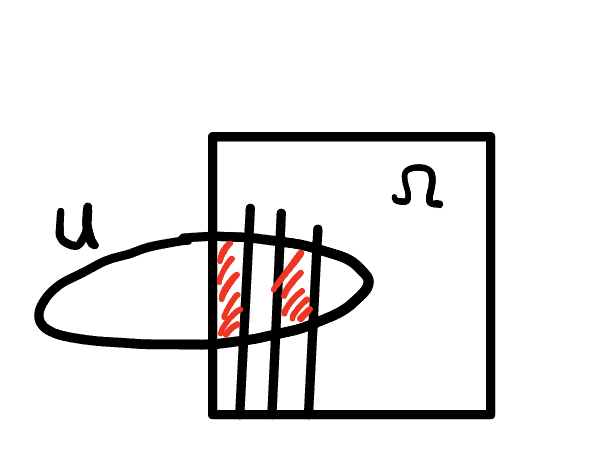
\includegraphics[width=0.2\textwidth]{lem.jpg}
  \caption{例: $\Omega \cap U$有多个连通分支}
\end{figure} 
\begin{proof}
    首先, $V \subsetneq U$ 为开集. 
    注意到, 
    $$ \partial \left( \Omega \cap U \right)=\partial U \cap \overline{\Omega}  \cup \left( \partial \Omega \cap U \right). $$ 
    若 $\partial V \cap U \cap \partial \Omega = \emptyset$, 则 
    $$ \partial V \subset \partial U \cap \overline{\Omega } \subset \partial U ,$$
    于是 $V \subset U$ 为闭集. 由于 $U$ 连通, 所以矛盾.  
\end{proof}
\begin{remark}
    \textcolor{purple}{上述集合运算是在全空间 $\cc^n$ 意义下进行的. 作为开子空间, $\Omega \cap U$ 仍是局部道路连通的, 所以 $V$ 为开集(从而也是 $\cc^n$ 的开集). 另外, 作为拓扑空间 $\Omega \cap U$ 的连通分支, $V$ 相对于 $\Omega \cap U$ 为闭(但不一定是在$\cc^n$中闭). 利用此信息结合假设$\partial V \cap U \cap \partial \Omega = \emptyset$, 可导出 $\partial V \subset \partial U \cap \overline{\Omega }$. }
\end{remark}

\begin{proposition}
    设 $\{K_j\}$ 为 $\Omega $ 中一列紧子集, s.t. $K_j \subset K_{j+1}^{\circ }, \Omega =\cup _j K_j$. 则 存在子列 $\{K_{j_{\nu }}\}$ 以及点列 $\{p_{\nu }\}$ s.t. $p_{\nu } \in K_{j_{\nu +1}}\setminus K_{j_{\nu }}$ 且 $\partial \Omega $ 包含于 $\{p_{\nu }\}$ 的极限点集.       
\end{proposition}
\begin{proof}
    将与 \(\partial\Omega\) 相交的、球心坐标以及半径均为有理数的球全体记为
\(
\{B_{\beta }\},
\)
其为可数集。

由于 \(\Omega\cap B_{\beta }\) 至多有可数个连通分支，故
\[
\mathcal{Q}
:=
\left\{
Q_\alpha:
Q_\alpha \text{ 为某个 } \Omega\cap B_{\beta }
\text{ 的连通分支}
\right\}
\]
为一个可数集。
由引理 \ref{lem4.4}\textcolor{purple}{(确保连通分支不是相对紧? 否则 $j_{\nu }$ 不能任意大)}，存在 \(p_1\in Q_1\)，使得
\[
p_1\in K_{j_1+1}\setminus K_{j_1}.
\]
同理，存在 \(p_2\in Q_2\)，使得
\[
p_2\in K_{j_2+1}\setminus K_{j_2},
\qquad
j_2\gg j_1.
\]
$\dots$\\
$\Rightarrow \exists p_{\nu }\in Q_{\nu }, p_{\nu } \in K_{j_{\nu }+1} \setminus K_{j_{\nu }}, j_{\nu } \geq j_{\nu -1}$. 则 $\{K_{j_{\nu }}\}$ 以及 $\{p_{\nu }\}$ 满足命题条件. 
\end{proof}

\begin{proof}[定理 \ref{thm4.1}, 全纯域 $\Rightarrow $ 全纯凸域]
    只要证 $\forall $ 紧 $K \subset \Omega $: 
    $$ d(\hat{K},\partial \Omega )  \geq d(K,\partial \Omega )~~ (>0) .$$
    ($\Rightarrow $ 等号成立. )   
    设
\[
0<\varepsilon<d(K,\partial\Omega).
\]
于是
\[
K_\varepsilon
:=
\left\{
z:d(z,K)\leq\varepsilon
\right\}
\subset\subset\Omega
\]
为紧集。
设
\[
r=(r_1,\ldots,r_n),
\qquad
r_j>0,
\qquad
\sum_j r_j^2=\varepsilon^2.
\]
则对任意 \(c\in K\)，有
\[
P(c,r)\subset B(c,\varepsilon)\subset K_\varepsilon \subset \subset\Omega.
\]
设 \(f\in\mathcal{O}(\Omega)\)，其在 \(P(c,r)\) 上有 Taylor 展开
\[
f(z)
=
\sum_\alpha
\frac{f^{(\alpha)}(c)}{\alpha!}(z-c)^\alpha.
\qquad (*)
\]
由 Cauchy 不等式，
\[
\left|
\frac{f^{(\alpha)}(c)}{\alpha!}
\right|
\leq
\frac{\sup_{K_\varepsilon}|f|}{r^\alpha}.
\]
于是, 其对任意 \(c\in\widehat{K}\) 也成立. 从而
\[
(*)\text{ 在 }P(c,r)\text{ 中内闭一致收敛},
\quad
\forall\,c\in\widehat{K}.
\]
因为
\[
B(c,\varepsilon)
=
\bigcup_{|r|=\varepsilon}P(c,r).
\]
所以 $f \in \mathcal{O}(B(c,\epsilon )), \forall c \in \hat{K}$. 因为 $\Omega $ 为全纯域, 所以存在 $f \in \mathcal{O}(\Omega )$ 其不能全纯延拓过任一个边界点, 于是 
$$ d(c,\partial \Omega ) \geq \epsilon , \quad \forall c \in \hat{K}. $$  
令
\[
\varepsilon \to  d(K,\partial\Omega).
\]
则
\[
d(c,\partial\Omega)\geq d(K,\partial\Omega),
\]
从而
\[
d(\widehat{K},\partial\Omega)
=
\inf_{c\in\widehat{K}} d(c,\partial\Omega)
\geq
d(K,\partial\Omega).
\]
\end{proof}

\begin{remark}
    实际上, 下面条件 
    $$ (A) \qquad \forall a \in \partial \Omega , \exists f \in \mathcal{O}(\Omega ), s.t. \text{其不能全纯延拓过} a $$
    可以推出全纯凸. 再结合 Cartan-Thullen 定理 $\Rightarrow (A) \iff $ 全纯域. 
\end{remark}

\begin{proposition}
    全纯域 $\Rightarrow $ 拟凸域. 
\end{proposition}
\begin{proof}
取紧穷竭列 \(\{K_j\}\)，使得
\[
K_j=\widehat{K_j},
\qquad
K_j\subset K_{j+1}^{\circ},
\qquad
\Omega=\bigcup_j K_j.
\]
固定 \(j\)。对任意
\(
a\in K_{j+2}\setminus K_{j+1}^{\circ},
\)
存在 \(f_a\in\mathcal{O}(\Omega)\)，使得
\[
\|f_a\|_{L^\infty(K_j)}<1,
\qquad
|f_a(a)|>1.
\]
取 \(a\) 的邻域 \(U_a\)，使得
\[
\inf_{U_a}|f_a|>1.
\]
由 Heine--Borel 定理，存在
\[
f_{j_1},\ldots,f_{j_{m_j}}\in\mathcal{O}(\Omega),
\]
使得
\[
\|f_{j_k}\|_{L^\infty(K_j)}<1,
\qquad \forall\,k,
\]
且
\[
\max_{1\leq k\leq m_j}|f_{j_k}|>1
\quad\text{于 }K_{j+2}\setminus K_{j+1}^{\circ}.
\]

用 \(f_{j_k}^{\,\nu}\)，其中 \(\nu\gg1\)，来代替 \(f_{j_k}\)，使得
\[
\sum_{k=1}^{m_j}|f_{j_k}|^2<2^{-j}
\quad\text{于 }~K_j,
\]
且
\[
\sum_{k=1}^{m_j}|f_{j_k}|^2>j
\quad\text{于 }~K_{j+2}\setminus K_{j+1}^{\circ}.
\]
因此
\[
\rho
:=
\sum_{j=1}^{\infty}
\sum_{k=1}^{m_j}|f_{j_k}|^2
\]
为 \(\Omega\) 上的 \(C^\infty\)  的 $\psh$  穷竭函数。
\end{proof}


\noindent\textbf{Levi 问题}: 拟凸域 $\Rightarrow $ 全纯域? (Oka 解决).

\begin{theorem}[H\"ormander]
    设 $\Omega \subset \subset \cc^n$ 拟凸, $\varphi \in \psh(\Omega )$, $v$ 为 $\Omega $ 上一个 $(0,1)$-形式, s.t. 
    $$ \db v =0 \quad (\text{分布意义})$$
    且 
    $$ \int_{\Omega } |v|^2 e^{-\varphi } <\infty . $$ 
    则 $\db u =v$ 在分布意义下存在解, s.t. 
    $$ \int_{\Omega } \left| u \right| ^2 \frac{e^{-\varphi }}{\left( 1+\left| z \right| ^2 \right)^2} \leq \int_{\Omega } |v|^2 e^{-\varphi } . $$
    若 $v \in C^{\infty }$, 则 $u \in C^{\infty }$. \textcolor{red}{(Carleman 方法)}      
\end{theorem}
\begin{remark}
    \textcolor{red}{涵盖了全纯、多次调和、拟凸。}
   \textcolor{purple}{ (证明可以参考陈伯勇: \textit{Cauchy-Riemann 方程的 $L^2$-理论}.)}
\end{remark}

\begin{proof}[Levi 问题]
    反证法. 假设 $\Omega $ 非全纯域. 则存在 $a \in \partial  \Omega $ 以及邻域 $U \ni a$, s.t. $\forall f \in \mathcal{O}(\Omega )$ 可全纯延拓至 $U$.      

    取 \(p\in \Omega\cap U\) 充分接近边界 \(\partial\Omega\)。
则存在
\[
p^*\in \partial\Omega\cap U,
\]
使得
\[
|p-p^*|=d(p,\partial\Omega).
\]
设 \(H\) 为过 \(p\) 与 \(p^*\) 决定的复直线，其横截 \(\partial\Omega\) 于 \(p^*\)。
不妨设
\[
p^*=0,
\qquad
H=\{z'=0\},
\qquad
z'=(z_1,\ldots,z_{n-1}).
\]
取
\[
f_0(z_n)=\frac{1}{z_n}.
\]
注意到: 若存在
\(
f\in\mathcal{O}(\Omega),
\)
使得
\[
f|_{\Omega\cap H}=f_0,
\]
则与假设矛盾(唯一性定理). 下面来证明 $f$ 的存在性. 

设
\(
\pi:\mathbb{C}^n\to\mathbb{C},
\,
z\mapsto z_n.
\)
取
\(
\chi\in C_0^\infty(\Omega ,\rr),
\)
使得 \(\chi=1\) 于 \(\Omega\cap H \subset \subset\Omega\) 中的一个邻域，
且
\(
\chi=0
\) 于 $\Omega\setminus \pi^{-1}(\Omega\cap H)$ 
中的邻域。
于是
\[
\pi^*f_0\in\mathcal{O}\bigl(\pi^{-1}(\Omega\cap H)\bigr),
\]
故
\[
\chi\cdot \pi^*f_0\in C_0^\infty(\Omega).
\]

令
\[
f:=\chi\cdot \pi^*f_0-u.
\]
为使 \(f\in\mathcal{O}(\Omega)\)，则 \(u\) 应满足
\[
\bar\partial u
=
\bar\partial\bigl(\chi\cdot \pi^*f_0\bigr),
\qquad
u|_{\Omega\cap H}=0.
\]
取
\[
\varphi(z)
=
2(n-1)\log|z'|+\lambda \circ \rho,
\]
其中 \(\rho\) 为 \(\Omega\) 上一个严格 $\spsh$  穷竭函数， \(\lambda\) 凸增。
当 \(\lambda\) 增长足够大时，
\[
\int_\Omega
\left|
\bar\partial\bigl(\chi\cdot \pi^*f_0\bigr)
\right|^2
e^{-\varphi}
<\infty. \quad (\text{\textcolor{red}{练习}})
\]
由 H\"ormander 定理, 方程 $\db u=\db \left( \chi \cdot \pi ^{*} f_{0} \right)$ 存在解, s.t. 
$$ \int |u|^2 \frac{e^{-\varphi }}{\left( 1+\left| z \right| ^2 \right)^2} <\infty . $$ 
因为 $u$ 在 $\Omega \cap H \subset \Omega $ 的某邻域上为全纯, 所以 
$$ u|_{\Omega \cap H}=0 \quad \textcolor{red}{(\text{练习})}. $$  
(因为 $\frac{1}{|z'|^{2n-2}} e ^{-\lambda \circ \rho }$ 有奇性.)
\end{proof}

\begin{remark}
    $$ \int_{\Gamma } \frac{\left| u \right| ^2}{|z'|^{2n-2}}=0 \, \Rightarrow u|_{\{z'=0\}}=0. $$
    (Laurent 级数.)
\end{remark}

\begin{definition}
    设 \(\Omega\) 为 \(\mathbb{C}^n\) 中一个区域，称
\(
\widetilde{\Omega}\subset\mathbb{C}^n
\)
为 \(\Omega\) 的一个（单叶）全纯包，若
\begin{enumerate}[(1)]
  \item 对任意
  \(
  f\in\mathcal{O}(\Omega),
  \)
  \(f\) 可全纯延拓至 \(\widetilde{\Omega}\)；

  \item \(\widetilde{\Omega}\) 为全纯域。
\end{enumerate}
\end{definition}

\begin{example}[Hartogs 圆]
    设 
    $$ H=\{(z_1,z_2) \in \cc^2: |z_1|<1, \frac{1}{2}<\left| z_2 \right| <1\} \cup \{(z_1,z_2): |z_1| <\frac{1}{2},|z_2|<1\} .$$
    则 $\widetilde{H}=\mathbb{D}^2:=\{(z_1,z_2):|z_1|<1,|z_2|<1\}$. 
\end{example}

一般地, 存在 $\Omega \subset \subset \cc^n$, s.t. 全纯包 $\widetilde{\Omega }$ 不存在.  

\begin{example}
设
\(
\Omega\subset\mathbb{C}^2
\)
为
\(
\left\{
|z_1|<1,\ |z_2|<2
\right\}
\)
去掉正方形
\(
I
=
\left\{
0 \leq  x_1<1, y_1=0, |z_2|\leq 1
\right\},
\)
\(
II
=
\left\{
0\leq y_1<1, x_1=0, 1\leq |z_2|<2
\right\}
\)
以及扇形
\(
S
=
\left\{
|z_1|<1, x_1\geq 0, y_1\geq 0, |z_2|<1
\right\}
\)
后所得区域。

\begin{figure}[htbp]
  \centering
  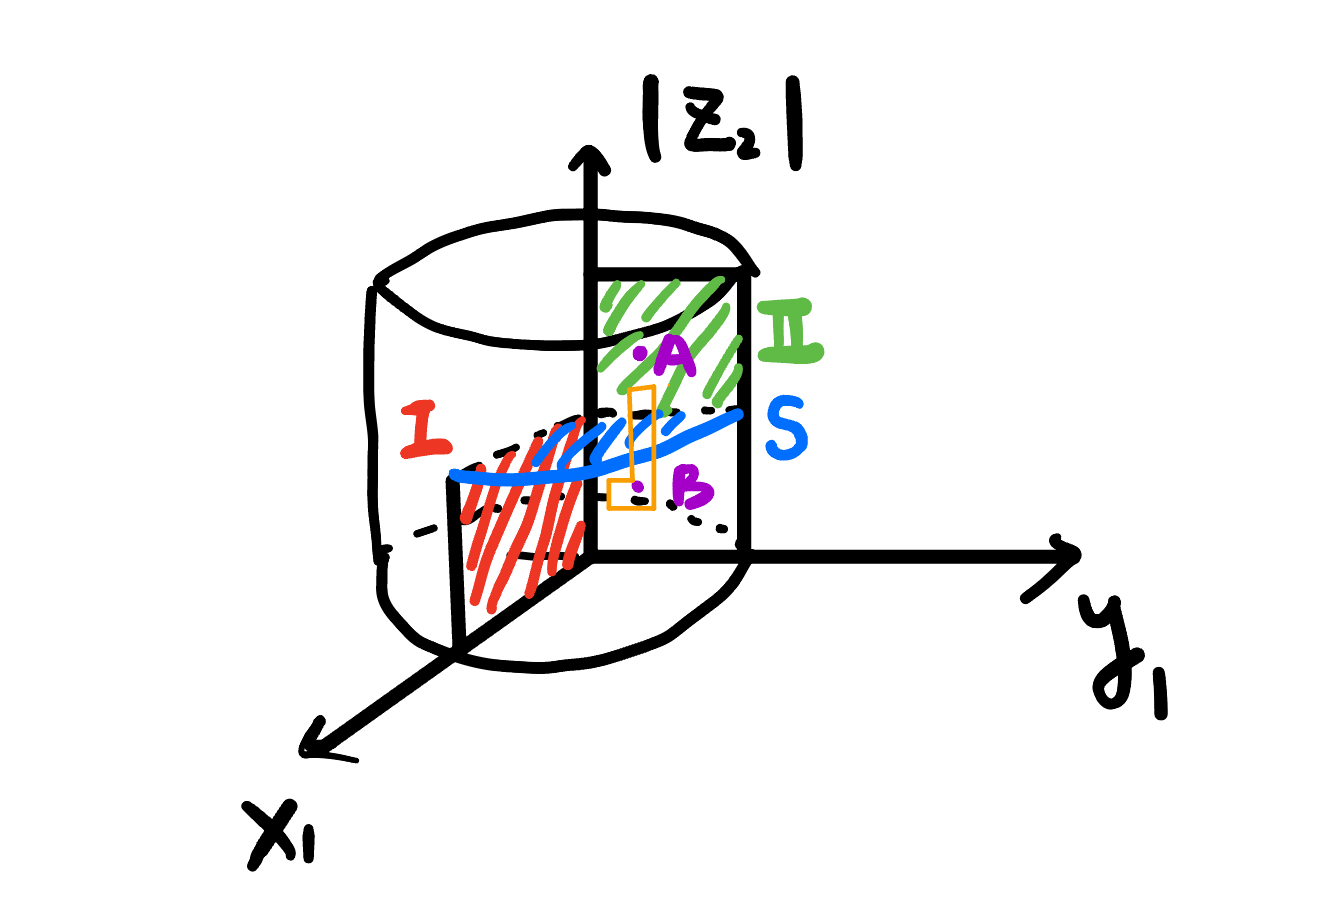
\includegraphics[width=0.4\textwidth]{Riemdom.jpg}
  \caption{$\Omega $ 不存在全纯包}
\end{figure} 
考察 \(\sqrt{z_1}\) 的单值支。
在 \(A,B\) 处取值符号相反。
另一方面，由 Hartogs 延拓，从 \(B\) 到 \(A\) 可延拓过 \(S\)。
因此，延拓后的函数在 \(A\) 处与 \(B\) 处取值相同
$\Rightarrow $  \(\sqrt{z_1}\) 的延拓为多值函数。
故 \(\widetilde{\Omega}\) 不存在！（\textcolor{red}{Riemann 域理论）}
\end{example}

